\documentclass[a4paper,10pt]{article}
\usepackage[utf8]{inputenc}
\usepackage[english,spanish]{babel}
\usepackage{amsmath}
\usepackage{fancyhdr}
\usepackage{amssymb}
\usepackage{graphicx}
\usepackage[hidelinks]{hyperref}
\usepackage{fancyhdr}
\usepackage{geometry}
\usepackage{enumitem}
\usepackage{titlesec}
\usepackage{caption}
\usepackage{float}
\usepackage{cite}
\usepackage[round]{natbib}
\usepackage{etoolbox}
\usepackage{lipsum}

% Configuración de la página
\geometry{top=2.5cm,bottom=2.5cm,left=2cm,right=2cm}

% Configuración del tamaño de los títulos
\titleformat{\section}{\normalfont\fontsize{14}{16}\bfseries}{\thesection.}{1em}{}
\titleformat{\subsection}{\normalfont\fontsize{12}{16}\bfseries}{\thesubsection.}{1em}{}
\titleformat{\subsubsection}{\normalfont\fontsize{11}{16}\bfseries}{\thesubsubsection.}{1em}{}

% Configuración de figuras y tablas
\renewcommand\spanishtablename{Tabla}
\captionsetup[table]{labelfont=bf,labelsep=period,justification=centering}
\captionsetup[figure]{labelfont=bf,labelsep=period,justification=centering}

% Configuración de encabezado y pie de página
\usepackage{fancyhdr}
\pagestyle{fancy}
\fancypagestyle{firstpage}{%
  \renewcommand{\headrulewidth}{0pt}%
  \fancyhf{}%
  \fancyhead[C]{%
        \small\scshape{1° REVISTA INGENIERÍA, MATEMÁTICAS Y CIENCIAS DE LA INFORMACIÓN (2022)}%
  }%
}

% Configuración de abstract
\renewenvironment{abstract}
 {\small
  \begin{center}
  \bfseries \abstractname\vspace{-.5em}\vspace{0pt}
  \end{center}
  \list{}{%
    \setlength{\leftmargin}{4mm}% <---------- CHANGE HERE
    \setlength{\rightmargin}{\leftmargin}%
  }%
  \item\relax}
 {\endlist}

\providecommand{\keywords}[2]
{
  \hfill \break
  \small	
  \textbf{\textit{#1:}} #2
}

% Añade esto al preámbulo
\usepackage{authblk}
\renewcommand\Authsep{, }
\renewcommand\Authands{, }
\renewcommand{\Affilfont}{\fontsize{8}{10}\selectfont\bfseries}
\renewcommand{\Authfont}{\fontsize{12}{10}\selectfont}
\setlength{\parskip}{0.5\baselineskip}%
\setlength\parindent{0pt}
\renewcommand{\headrulewidth}{0pt}
\renewcommand{\footrulewidth}{0pt}

\usepackage{xpatch}

\makeatletter
\xpatchcmd{\@maketitle}
  {\@title}
  {\fontsize{17}{20}\selectfont\bfseries\@title}
  {}{}

\let\@ssect@ORIG\@ssect
\let\@runin@ssect\@ssect

\apptocmd{\@runin@ssect}{%
  \addcontentsline{toc}{subsubsection}{%
    % Comment out the following line to remove “phantom number” indentation in
    % the TOC
    \protect\numberline{}% no number in TOC
    #5% the title
  }%
  \let\@ssect\@ssect@ORIG       % restore the normal \@ssect
}{}{\FAILED}

\newcommand*{\runinsubsection}{%
  \let\@ssect\@runin@ssect
  \@startsection{subsubsection}%
  {2}% level
  {\z@}% indentation of heading from the left margin
  {-3.25ex\@plus -1ex \@minus -.2ex}% absolute value = beforeskip
  {-0.5em \@plus -.1em}% when negative, opposite = skip to leave right of a
                       % run-in heading.
  {\normalfont\large\bfseries}% style
  *% we want an unnumbered subsection
}
  
\makeatother
% Modifica esta parte para definir los autores, afiliaciones y correos
\title{CLOUD COMPUTING: RETOS Y OPORTUNIDADES}
\author[1,*]{Silvana Yanira Daza Santos}
\author[2]{Wellington Bienvenido Muñoz Cedeño}
\affil[1]{Universidad Laica "Eloy Alfaro" de Manabí, El Carmen, Ecuador}


% Título de la cabeceras, reducir en caso que el título sea muy largo
\newcommand\shorttitle{CLOUD COMPUTING: RETOS Y OPORTUNIDADES}
% Autores para las cabeceras - sólo apellidos, et al. si hay más de 3
\newcommand\authors{CLOUD COMPUTING: RETOS Y OPORTUNIDADES}
\fancyhf{}
\renewcommand\headrulewidth{0pt}
\fancyhead[C]{%
\ifodd\value{page}
  \small\scshape\shorttitle
\else
  \small\scshape\authors
\fi }

\fancyhead[R]{\thepage\ifodd\value{page}\else\hfill\fi}

\date{}


\begin{document}

\maketitle
\thispagestyle{firstpage}
%\thispagestyle{empty} % Para no numerar la primera página

\begin{abstract}
Este trabajo ha explorado las oportunidades y desafíos del cloud computing, así como su nomenclatura y antecedentes. Las ventajas de la computación en la nube son evidentes para empresas, organizaciones públicas y usuarios, destacándose su rapidez, flexibilidad y disponibilidad. Estas ventajas abarcan aspectos económicos, tecnológicos, ambientales y sociales, siendo el ahorro en costos y la facilidad de ampliar recursos las más significativas para los usuarios.     

\keywords{Palabras claves}{Computación en la nube, Escalabilidad, Seguridad de datos, Disponibilidad del servicio, Almacenamiento distribuido, Privacidad, Proveedores de servicios, Innovación tecnológica. }
\end{abstract}

\selectlanguage{english}
\begin{abstract}
This work has explored the opportunities and challenges of cloud computing, as well as its nomenclature and background. The advantages of cloud computing are evident for companies, public organizations and users, highlighting its speed, flexibility and availability. These advantages cover economic, technological, environmental and social aspects, with cost savings and the ease of expanding resources being the most significant for users.  

\keywords{Keywords}{Cloud Computing, Scalability, Data Security, Service Availability, Distributed Storage, Privacy, Service Providers, Technology Innovation.}
\end{abstract} 

\selectlanguage{spanish}
\section{Introducción}
La computación en la nube es un modelo que permite acceder a recursos compartidos, como redes y servidores, de manera flexible y eficiente, con mínima gestión por parte del proveedor. Este modelo ofrece ventajas significativas, como economías de escala, que reducen la necesidad de grandes inversiones en tecnologías de la información, convirtiendo a los proveedores en utilities que facilitan el acceso a la capacidad computacional bajo demanda. A lo largo del artículo se explorarán estas y otras ventajas, aunque el aprovechamiento efectivo de estas tecnologías enfrenta desafíos tecnológicos, legislativos y políticos que deben ser abordados para satisfacer la creciente demanda.


\section{Denominación}
La computación en la nube, también conocida como cloud computing, se refiere a la entrega de servicios tecnológicos bajo demanda, eliminando la necesidad de instalar y mantener software localmente. Este enfoque está transformando la forma en que se gestiona la informática, ya que permite acceder a programas y datos a través de Internet, como es el caso de Google Docs, que ofrece herramientas de productividad sin necesidad de instalación en el equipo del usuario.

La transición hacia la nube es un proceso que aún se encuentra en sus primeras etapas, pero está teniendo un impacto significativo, especialmente en las industrias tecnológicas de la llamada Cuarta Revolución Industrial. Aunque el software tradicional sigue siendo predominante, las innovaciones en la computación en la nube están ganando terreno rápidamente.

La adopción de la nube está cambiando la informática desde el escritorio hacia servicios remotos, afectando a todos los niveles de uso, desde usuarios ocasionales hasta desarrolladores y administradores de TI. Este cambio recuerda a la llegada de las computadoras personales en los años 80, cuando los usuarios obtuvieron más control sobre su entorno informático. Ahora, con la computación en la nube, la infraestructura y los datos se gestionan en centros de datos externos, accediendo a ellos a través de Internet.

A diferencia de los sistemas tradicionales de tiempo compartido, donde un servidor central controla los recursos, la nube permite que múltiples servidores trabajen de manera colaborativa e intercambien datos. Esto representa un cambio de paradigma en la forma en que los usuarios y administradores gestionan y controlan los recursos informáticos, cediendo en muchos casos este control a proveedores externos de servicios en la nube.

Este modelo tiene ventajas claras: elimina la necesidad de instalar, configurar y actualizar software localmente, además de mantener la infraestructura necesaria. Subcontratar la computación a servicios en la nube permite a las empresas centrarse en su actividad principal y mejora la colaboración y movilidad, ya que los usuarios pueden acceder a sus datos y aplicaciones desde cualquier lugar.

Desde la perspectiva de Google, se destacan seis características clave de la computación en la nube: se centra en el usuario, facilitando el acceso y el intercambio de datos; se enfoca en tareas, priorizando lo que el usuario necesita hacer; es poderosa, con capacidad de procesamiento superior a la de una computadora individual; es accesible, permitiendo acceder a información desde múltiples ubicaciones; es inteligente, utilizando análisis de datos avanzados; y es programable, automatizando tareas para proteger la integridad de los datos y optimizar su gestión.

\begin{figure}[h!]
    \centering
    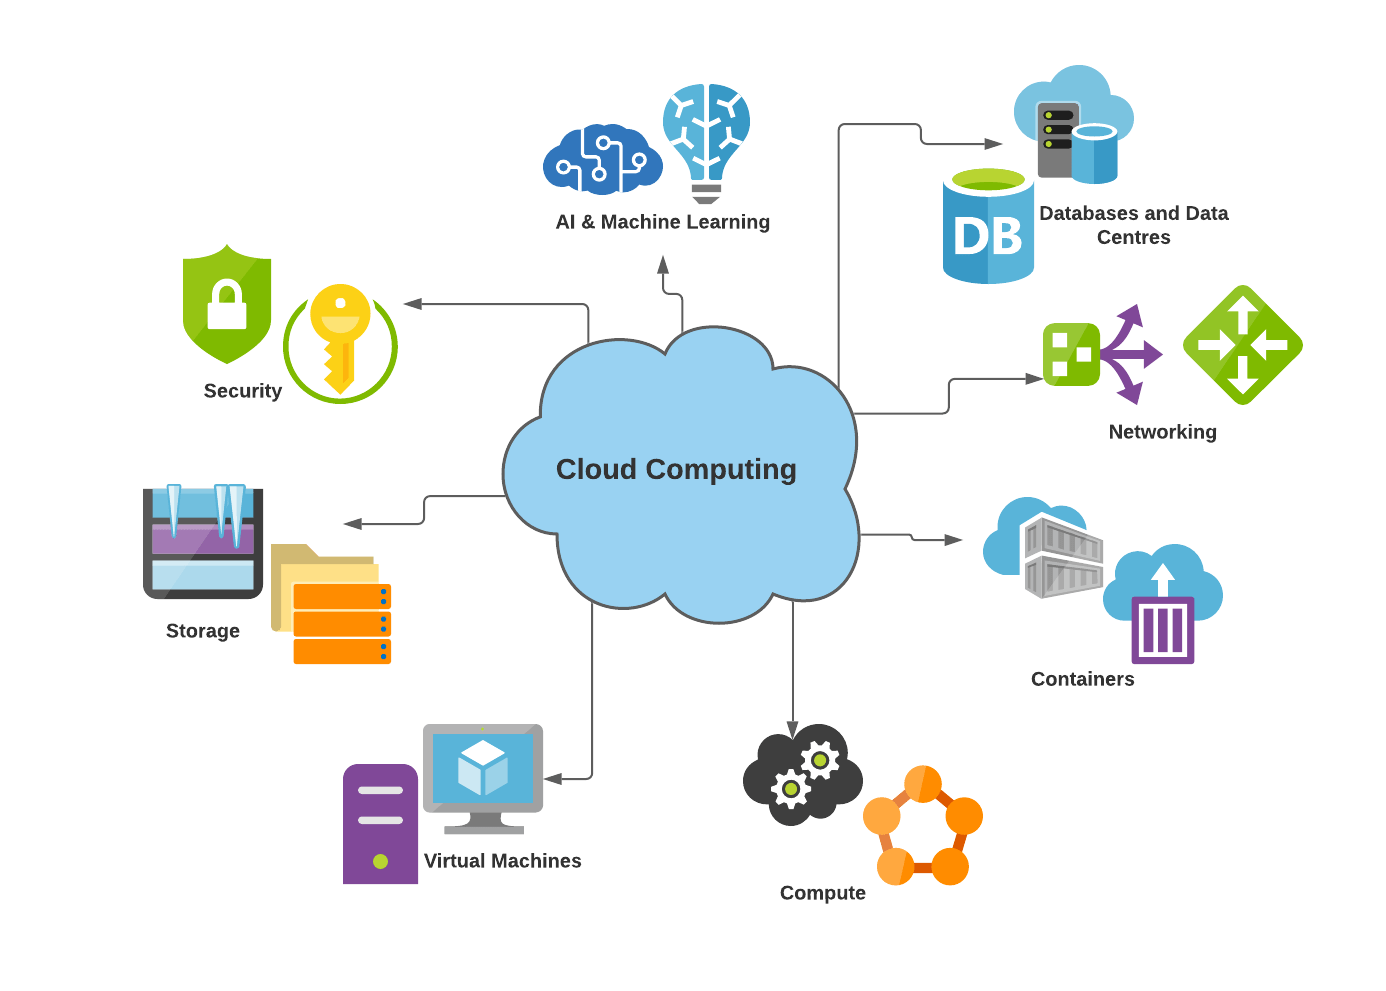
\includegraphics[width=0.5\linewidth]{Cloud-Computing.png}
        \caption{Cloud-Computing}
    \label{fig:ejemplo}
\end{figure}

Además, la nube fomenta la innovación al reducir costos y facilitar el desarrollo de nuevos productos y servicios, mejora la productividad al permitir el acceso remoto a los recursos, y ofrece ventajas técnicas al mantener a los usuarios actualizados con la última tecnología. Los proveedores de servicios en la nube también ofrecen mayor resiliencia ante desastres y recuperación eficiente, ya que controlan directamente la infraestructura que utilizan sus clientes.


\section{Retos y Oportunidades}
Según un estudio de la Universidad de Berkeley, el cloud computing enfrenta diez desafíos principales: disponibilidad del servicio, problemas con el bloqueo de datos, confidencialidad y capacidad de auditoría de los datos, cuellos de botella en la transferencia de datos, rendimiento impredecible del servicio, escalabilidad del almacenamiento, tolerancia a fallos en sistemas distribuidos, rápida escalabilidad tecnológica, reputación afectada y licencias de software.

A pesar de estos desafíos, el cloud computing ofrece a las organizaciones acceso flexible a la información, mayor interacción entre los participantes, reducción de costos y acceso a recursos disponibles. Sin embargo, el reto principal es mantener estos beneficios a largo plazo.

Para los proveedores de software, cambiar las operaciones a la nube implica ventajas, como desarrollar, probar y ejecutar software en plataformas elegidas por el proveedor, con actualizaciones rápidas. Sin embargo, aún persisten desafíos, como la diversidad de entornos operativos con los que deben interactuar.

La necesidad de construir y mantener centros de datos ha generado una expansión de proveedores que ofrecen infraestructura. Amazon Web Services (AWS) y Google con su App   , son ejemplos de empresas que proporcionan capacidad informática y almacenamiento según demanda. Esto facilita la implementación de software en la nube, pero también presenta desafíos de escalabilidad, ya que los sistemas deben funcionar sin problemas incluso con un aumento de usuarios y la información procedente de múltiples fuentes.

\begin{figure}[h!]
    \centering
    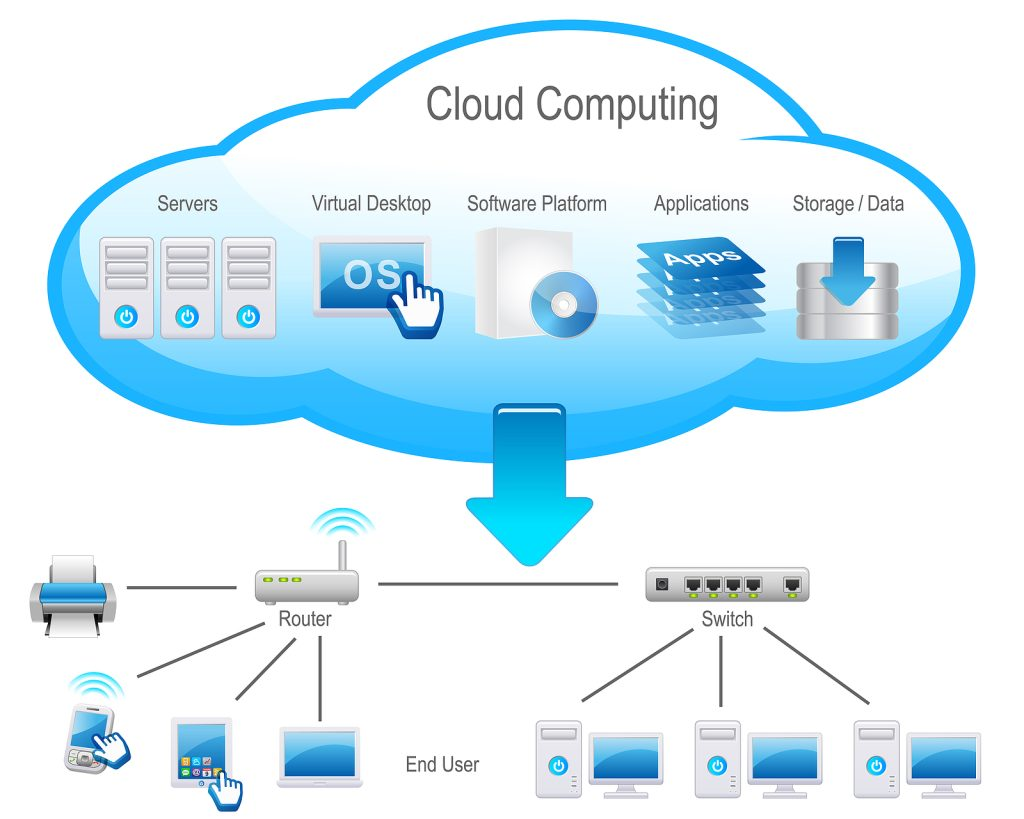
\includegraphics[width=0.5\linewidth]{Cloud-computing-challenges-and-opportunities.jpg}
        \caption{Cloud computing retos y oportunidades}
    \label{fig:ejemplo}
\end{figure}


La interfaz basada en navegadores también tiene retos. Duplicar la funcionalidad de sistemas operativos modernos en un navegador web es difícil, y se necesita dominar diversos lenguajes de programación y entornos operativos. Los desarrolladores deben integrar bases de datos, servidores y clientes usando múltiples lenguajes, como SQL, JavaScript y PHP, lo que añade complejidad.

La computación en la nube plantea desafíos para la privacidad y seguridad. Permitir a terceros gestionar datos personales genera preguntas sobre control y propiedad, así como la posibilidad de pérdida de acceso a los documentos si se cambian proveedores o no se paga el servicio. La privacidad y la capacidad de respuesta ante órdenes judiciales también son preocupaciones importantes, ya que es menos probable que un proveedor de servicios defienda los derechos del usuario.




\section{Conclusiones}

La computación en la nube está transformando la informática al trasladar aplicaciones y documentos del escritorio a una infraestructura basada en la web, permitiendo a los usuarios acceder a ellos desde cualquier dispositivo con conexión a Internet. Esto no solo facilita el trabajo remoto, sino que también fomenta la colaboración grupal, ya que varios usuarios pueden trabajar en los mismos documentos y programas desde distintas ubicaciones. Además, la nube ha evolucionado como un modelo dominante para la entrega escalable de recursos de TI, como servidores y almacenamiento, que son accesibles bajo demanda.

A pesar de sus beneficios, como el impulso de tendencias tecnológicas clave, incluyendo el Internet de las cosas, la computación móvil, los macrodatos y la inteligencia artificial, la computación en la nube también presenta desafíos. Entre los más significativos está la protección de los datos de los usuarios, una preocupación que sigue siendo central a medida que la dependencia de estos servicios continúa creciendo en nuestra vida diaria.


% \bibliographystyle{plain}
\bibliographystyle{plainnat}
\bibliography{bibliografia}

[1] NIST. Cloud computing. https: //www.nist.gov/.2011.

[2] B. Hayes. Portal The ACM Digital Library. Volume 51, N 7. https: //dl.acm.org/doi/fullHtml/10.1145/1364782.1364786. 2008.

[3] T. Nelson. Computer Lib/Dream Machines. ISBN10: 0486819558. 1974

[4] A. Benlian, T. Hess. Opportunities and risks of software-as-a-service: findings from a survey of IT executives. Decis Support Syst 52(1): 232–246. 2011.

[5] O. Arasaratnam. Introduction to cloud computing. In: Halpert B (ed) Auditing cloud computing, asecurity and privacy guide. Wiley, Hoboken, NJ,
pp 1–13. 2011.

\section *{Anexo: Enlace al repositorio }
 \href{}{Repositorio GitHub: Cloud computing: retos y oportunidades}

\end{document}